In this section, we briefly explained the planned implementation, integration and testing of system components. 

\subsection{Implementation}
\indent The system is structured around three primary layers: client, business, and data. These will be concurrently developed and later integrated. By doing so, each layer can be tested individually, and after integration, comprehensive system-wide testing can be conducted. We will employ a hybrid strategy, combining bottom-up and thread methodologies, to leverage the advantages of both.
\\
\indent The thread approach aids in creating interim deliverables for stakeholder evaluation, proving extremely beneficial for system validation. Concurrently, the bottom-up strategy facilitates incremental integration, enhancing bug detection by allowing for the testing of subsystems as they progressively evolve through the addition of new modules.
\\
\indent The thread strategy involves pinpointing the system's functionalities and the specific segments of the components (termed as sub-components for practical purposes, though they may not align precisely with design sub-components) that are responsible for these functionalities. Since multiple sub-components collaboratively contribute to a single function, it's crucial to establish a sequence for their implementation, for which the bottom-up approach is particularly useful.
\\
\indent This mixed strategy enables the allocation of different feature implementations to independent development teams working in parallel. However, it's essential to identify any common components beforehand to prevent duplication of efforts in creating the same component or sub-component more than once. This approach not only streamlines the development process but also ensures a more efficient and organized integration of the various system parts.

\subsubsection{Client Application}
Static parts of Client Web Application ,in other words Frontend, can be implemented without server side implementation. Mockups and UI-UX design can be used for this development. However, dynamic actions rely on REST API to communicate server-side responsible for business logic. So, using documentation, unit test mocking REST API can be used to implement Frontend code.
\subsubsection{Application Server}
Application Server, in other words Backend, is responsible for the business logic in server side. We can separate some parts of the Application Server to be developed in parallel.
The components to be incorporated into the system are derived directly from the system's requirements. The developers can be work separately on these components and integrate and test at the end of their development the components to evaluate the dependency and the interactions between them. The entire business logic can be tested separately from the client logic, which accelerates the development process. Below is a concise summary of the system's components with priorities.
\begin{tabularx}{0.8\textwidth} { 
  | >{\raggedright\arraybackslash}X 
  | >{\centering\arraybackslash}X 
  | >{\raggedleft\arraybackslash}X | }
 \hline
\textbf{Component} & \textbf{Importance} &  \textbf{Complexity} \\
 \hline
 Authentication Manager  & High  & Low  \\
  \hline
 Profile Manager  & Medium  & Low  \\
\hline
 Tournament Manager  & High  & High  \\
\hline
 Battle Manager  & High  & High  \\
\hline
 Team Manager  & Medium  & Low  \\
\hline
 Notification Manager  & Low  & Medium  \\
\hline
 Repository Components  & High  & Medium  \\
\hline
 Submission Manager  & High  & Medium  \\
\hline
 Github Manager  & Low  & Low  \\
\hline
 Scoring Manager  & High  & High  \\
\hline
 File Manager  & Medium  & Low  \\
\hline
\end{tabularx}

So, briefly, we have to consider the importance and complexity of a component before starting to implement the component. This kind of analysis enables us to estimate time and work cost spent for a certain part of application.
\\

\subsubsection{Implementation Plan}
\begin{enumerate}
    \item \textbf{Repository Components:} For the application, data access layer has a great importance because all other components mainly rely on data access at some point. Database interaction is crucial because of the CRUD operations. So Tournament, Battle, User, Team and Submission Repository components are implemented firstly in parallel because there is no dependency between them.
    \item \textbf{Notification Manager:} Even though a notification system is not a crucial part of the system, it's methods widely used by lots of components, so implementing it at early stages can be very helpful to see its usage among other components when implementing them. EmailManager and InAppNotificationManager are another required components for the Notification Component and they are considered within Notification Manager Component.
    \item \textbf{Authentication Manager:} This component offers 2 interfaces which is related to users' authentication. \textbf{Registration, login and logout} functionalities are very fundamental to operate all business logic. Also it provides a session manager interface which is used by other components in which it is important to know who the user is, what type it is and what permissions it has.
    \item \textbf{Tournament Manager:} Implementation of this component  can be at the end if we follow just bottom-up approach. However, one of our goals is to create intermediate products and this component, even if it is a complex component, can helps us to create such an intermediate product. It has also no dependency other than Tournament Repository, Notification Manager and Authentication Manager.
    \item \textbf{File Manager:} This component mainly responsible to communicate with File Storage Service. It encapsulate the operations such as fetch,read or write file from or to the file system on the cloud. It provides an interface to manage files so it is needed by other components.
    \item \textbf{Profile Manager:} Unlikely to Tournament, this component has really low complexity without no real dependency other than repositories. By implementing Profile Manager at early stages, we can achieve a intermediate product with less effort and no dependency is needed.
    \item \textbf{Scoring Manager:} Again this is another components which is responsible to communicate to an external service. Also it provides an iterface to calculate score of a submission. This component also has high priority with its required components such as Sandbox Manager and Static Analysis Manager.
    \item \textbf{Github Manager:} Even though Github Manager is not fundamental as some main components such as Submission Manager and Battle Manager, implementing it early comes with advantages. It provides interfaces to these components. Also there can be another components using some logic related to Github. 
    \item \textbf{Submission Manager:} This component is one of the main components in the application which provides Submission related methods. It is very critic to use because it also provides an endpoint to be triggered by Github. 
    \item \textbf{Team Manager}: It provides interface related to team operations. Needed from Battle Manager.
    \item \textbf{Battle Manager:} This components provides the endpoints about Battles and operates the logic related to Battles. It uses various interfaces from various components so it is good to implement this component at the last stages.
\end{enumerate}

\newpage
\subsection{Integration \& Testing}
\indent The section describes the integration plan of the different components and subcomponents of the CodeKataBattle. The provided graphs illustrate the interdependencies between various components and subcomponents. Before any subcomponent is combined with others to create a larger component, it must undergo unit testing. Following this integration, the complete component is then subjected to further testing.
\\
\indent Before proceeding with the integration testing of a component, it is crucial to satisfy two key conditions, each with its distinct benefits. The first condition is that the component's interface must encompass all the functionalities detailed in the component interface diagram. This ensures that the component adheres to the predefined design specifications, which is vital for maintaining consistency and predictability in the system’s overall behavior. Adhering to these specifications also facilitates easier integration with other components, as each piece is designed to fit seamlessly within the broader system architecture.
\\
\indent The second prerequisite is that the component must successfully clear all unit tests. Unit testing plays a critical role in verifying that each individual part of the component functions as intended in isolation. This process helps in identifying and rectifying any bugs or issues at an early stage, significantly reducing the risk of defects in the later stages of development. Successful unit testing guarantees a higher level of reliability and stability in the component, which in turn contributes to the robustness of the final integrated system. By ensuring that each component is thoroughly tested and fully functional before integration, the overall quality and performance of the system are enhanced, leading to a more efficient, reliable, and effective product.
\\
\indent As you can see the diagrams below, Driver is used as unit test to mock the not-finished components. This part is crucial during the integration test written here should be passed. 

\newpage
\indent First integration to be handled is integrating \textbf{Repository Components} to DBMS in order to sustain a working data access layer. To enable other components to handle data this integration is very crucial. This is a prelimanary integration with DBMS. Unit Testing is used to mock the  other components being under development. This Driver is mainly responsible to mock repository calls from the components using them. Moreover, it checks the validity of the results.

\begin{figure}[H]
    \centering
    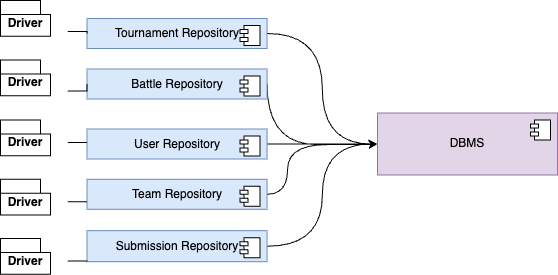
\includegraphics[width=\linewidth]{Images/integration/integration_1.drawio.png}
    \caption{Integration of Repository Components}
\end{figure}

\newpage
\indent Notification subsystem is integrated then to be used by other following components. It is very crucial here, after implementing EmailManager and InAppNotificationManager according to the external APIs, NotificationManager is implemented because there exists a dependency between NotificationManager and other two components. Testing is done as explained above with mocking usage of notification according to INotificationManager interface documentation. 

\begin{figure}[H]
    \centering
    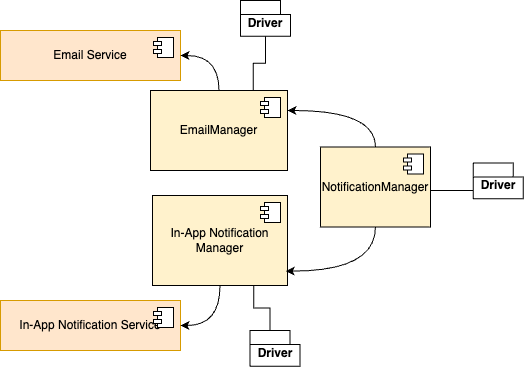
\includegraphics[width=\linewidth]{Images/integration/integration_2.drawio.png}
    \caption{Integration of Notification Subsystem}
\end{figure}

\newpage
\indent Authentication Manager is the component responsible for authentication operations. Its integration is done after implementing user repository and notification subsystem. In this stage of development, we are able to implement functions mocked for User Repository and Notification subsystem. Naturally, Unit tests must be passed before and after integration of Authentication Manager Component to these components. At this point, we also have some endpoints to Client Application after integration, so we can do Register, Login, Logout operations end-to-end. Application Server is developing independently, so we will use and test endpoints with the help of some tools such as Postman. At this time, it would be very helpful to start a Postman collection to document the endpoints.

\begin{figure}[H]
    \centering
    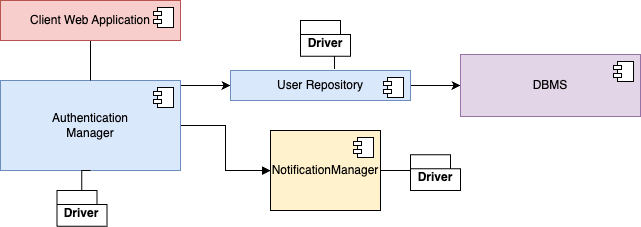
\includegraphics[width=\linewidth]{Images/integration/integration_3.drawio.png}
    \caption{Integration of Authentication Manager Component}
\end{figure}

\newpage
\indent Tournament Manager helps us to create an intermediate product because it has very few dependencies. At this stage, we integrated it to developed parts of application. Unit tests must be passed before and after integration. There will be some operations requires to send notification via email and in-app notification. Especially, for Notification Subsystem, implementing this functions must be aligned with unit tests. 

\begin{figure}[H]
    \centering
    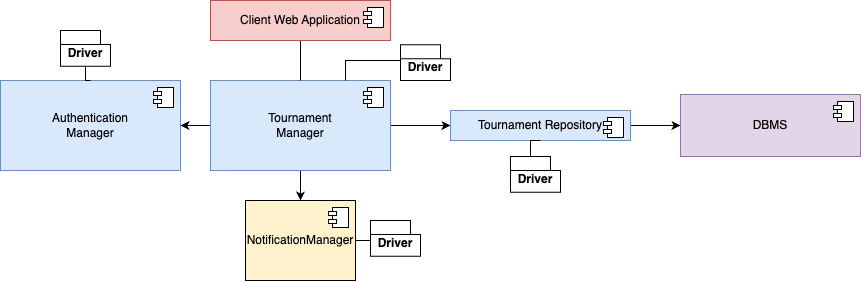
\includegraphics[width=\linewidth]{Images/integration/integration_4.drawio.png}
    \caption{Integration of Tournament Manager Component}
\end{figure}

\newpage
\indent File Manager can be developed and integrated to File Storage Service independently. This is also can be done in parallel to other components above. 

\begin{figure}[H]
    \centering
    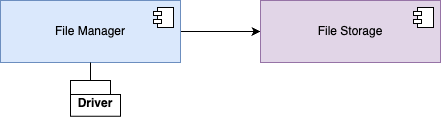
\includegraphics[width=\linewidth]{Images/integration/integration_5.drawio.png}
    \caption{Integration of File Manager Component}
\end{figure}

\newpage
\indent Profile Manager is another component to help to create intermediate product with the components Authentication Manager and Tournament Manager. It is integrated to User Repository and File System Manager for the profile specific operations. Also similar to Tournament Manager it uses session information from Authentication Manager and dependent on it. File Manager is integrated to all system via Profile Manager at this stage.

\begin{figure}[H]
    \centering
    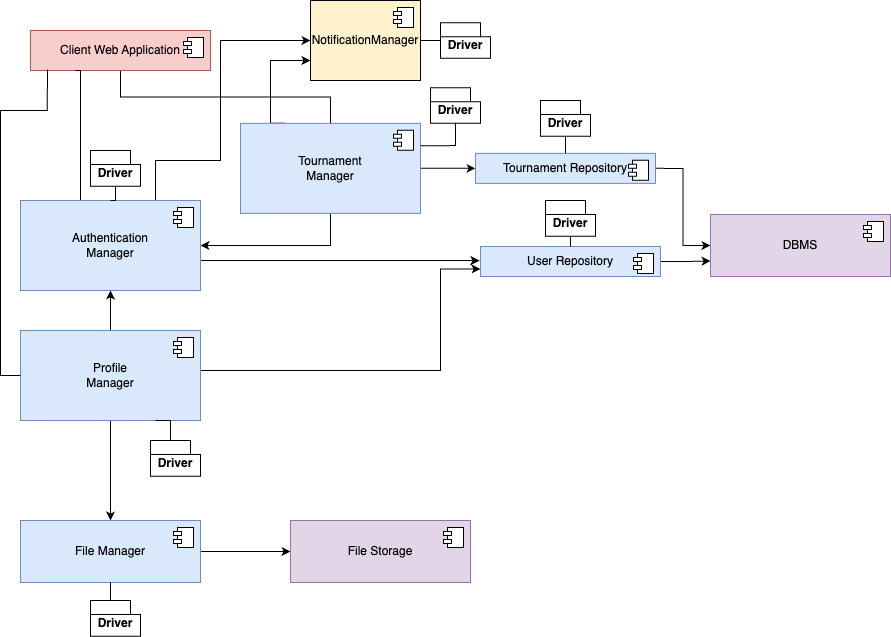
\includegraphics[width=\linewidth]{Images/integration/integration_6.drawio.png}
    \caption{Integration of Profile Manager Component}
\end{figure}

\newpage
\indent Scoring Manager and Github Manager can be implemented and integrated in parallel. For Scoring Manager, there are two other components which are responsible to Sandbox Manager and Static Analysis Manager. Firstly, Static Analysis Manager is integrated to 3rd Party API, then it is integrated to Scoring Manager with Sandbox Manager. Also Github Manager is integrated to Github with necessary documentation provided by Github.

\begin{figure}[H]
    \centering
    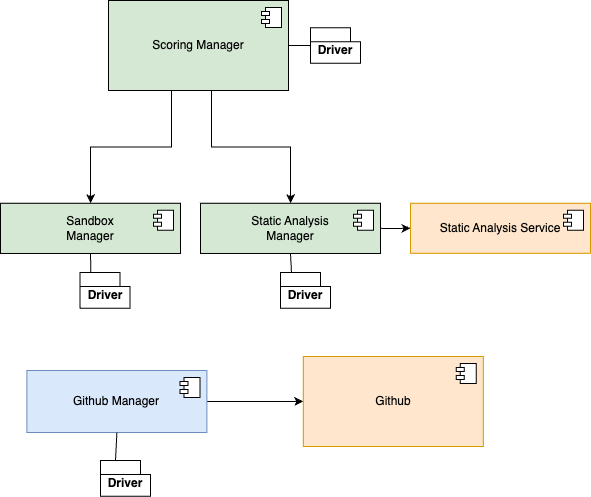
\includegraphics[width=\linewidth]{Images/integration/integration_7.drawio.png}
    \caption{Integration of Scoring and Github Manager}
\end{figure}

\newpage
\indent Submission Manager has a dependency over Scoring Manager, Github Manager and File Manager. Its implementation and integration will be held after these components. Also, usage of these components' provided interfaces from Submission Manager should be aligned with unit test written before for these components. Submission Manager is still sperated from the application because mainly Battle Manager uses the interface provided by Submission Manager.

\begin{figure}[H]
    \centering
    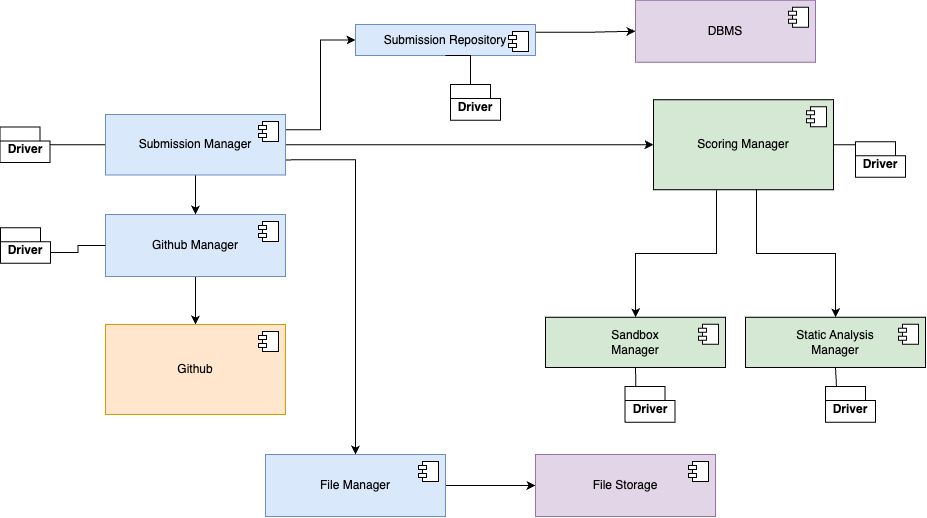
\includegraphics[width=\linewidth]{Images/integration/integration_8.drawio.png}
    \caption{Integration of Submission Manager}
\end{figure}

\newpage
\indent At the end Battle Manager, which uses repository components, scoring and Github related actions via Submission Manager and session methods, is implemented and integrated. Of course, Team Manager is firstly implemented and integrated to Battle Manager with the help of  some unit test. Then Battle Manager integrated to Submission Manager, Authentication Manager, Repository Components, File Manager and Notification Manager. As you can see, it needs lots of components to be implemented to  operate and be integrated to application. 

\begin{figure}[H]
    \centering
    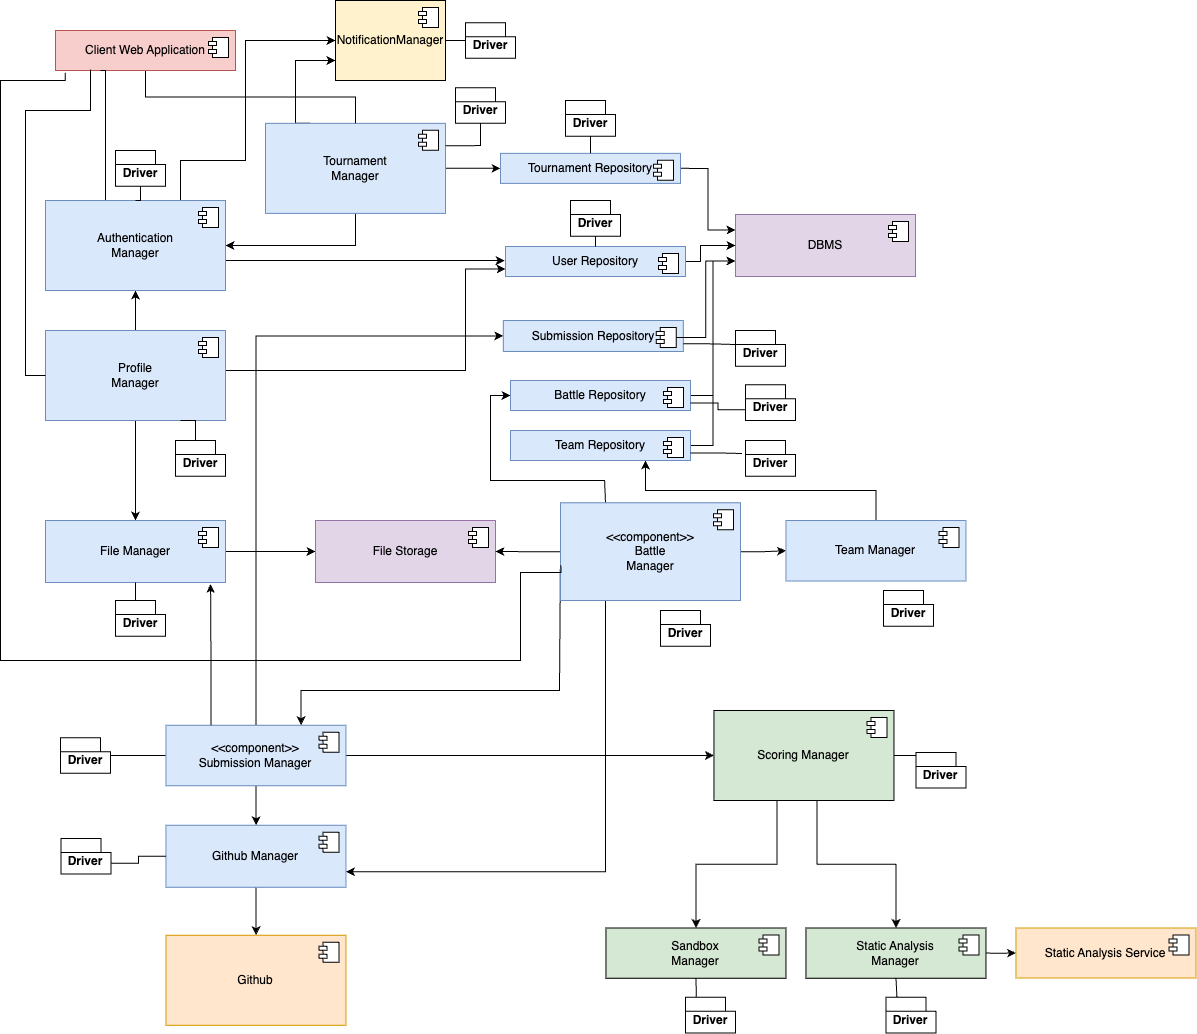
\includegraphics[width=\linewidth]{Images/integration/integration_9.drawio.png}
    \caption{Integration of Battle and Team Manager}
\end{figure}

\newpage
\subsection{Testing}
\indent CodeKataBattle is subjected to a comprehensive list of testing activities, each varying in scope and detail. In the development stage, it is crucial to test every component or module individually to ensure its functionality aligns with expectations. 
\\
\indent Given that some components might not function independently, the creation of Driver components becomes necessary. These components simulate the operations of adjacent modules, encompassing both normal and aberrant behaviors, to assess the robustness of each component.
\\
\indent Once individual components have been satisfactorily tested, the next phase involves their integration and the testing of this integrated setup. The CodeKataBattle system employs a blend of bottom-up and thread strategies for this process, as previously discussed. 
\\
\\ To comply with requriements discussed in RASD, system must be tests as a whole. This final testing phase confirms that all features are correctly developed and meet both functional and nonfunctional requirements. System testing, being a black-box technique, should involve not just the developers but also the stakeholders.

\begin{enumerate}
    \item The system should be tested to understand whether all requirements are fulfilled or not. 
    \item Also, there can be some performance problem related to some inefficient code, algorithm or a bottleneck caused by a design choice. This kind of performance testing is important to simulate workload or traffic in order to find weak aspects of the application in terms of speed, memory, resource utilization etc.
    \item In some cases, user can behave differently from stakeholders or developers. To understand such cases, it can be helpful to test user actions with different scenarios, devices etc. 
    \item Moreover, it is helpful to make stress testing to see system's ability to recover from failures. The objective here is to ensure the system's resilience by pushing it beyond its normal operational capacities and observing how it recovers from failures. This involves overwhelming the system's resources or depriving it of them to test its limits and recovery capabilities.
\end{enumerate}

\indent Whenever new features are introduced to the system, testing is essential to identify any bugs. Additionally, the testing methods outlined above must be employed to ensure the system's proper functioning throughout the implementation phase. This early and continuous testing is crucial for prompt bug detection.
\\
\indent Feedback from users and stakeholders is equally important during system development. Initially, stakeholders should be briefed on the planned functionalities to ascertain if the system aligns with their expectations. Also, intermediate versions of the system should be shared with them for feedback on any issues and see the satisfaction.

\indent This process of receiving regular feedback is vital for the validation of the system throughout its development. It enables developers to promptly identify if the system meets the intended requirements and customer expectations. If discrepancies are found between the system’s current state and the stakeholders' expectations, developers can make necessary adjustments. This approach not only ensures the system's relevance and efficacy but also aligns its development closely with user needs and preferences.